\documentclass[10pt]{article}
\usepackage[left=2.54cm,top=2.54cm,right=2.54cm,bottom=2.54cm]{geometry}
\usepackage{fancyhdr}
\usepackage{afterpage}
\usepackage{setspace}
\usepackage{bibspacing}
\singlespacing

%%%% YOU CAN PUT YOUR OWN DEFINITIONS HERE
\newfont{\toto}{msbm10 at 12 pt}
\newfont{\ithd}{cmr9}
\newcommand{\equa}[1]{(\ref{eq:#1})}
\newcommand{\laeq}[1]{\label{eq:#1}}
\newcommand{\figu}[1]{\ref{fig:#1}}
\newcommand{\lafi}[1]{\label{fig:#1}}
\newcommand{\fmo}{\tilde{U}}
\newcommand{\fve}{\tilde{u}}
\newcommand{\Dt}{\Delta t}

\newcommand{\R}{\mathbb{R}}
\newcommand{\Z}{\mathbb{Z}}
\newcommand{\si}[1]{\rm\scriptscriptstyle{#1}}
%%%% END OF YOUR DEFINITIONS 

\pagestyle{fancyplain}
\renewcommand{\headrulewidth}{0pt}

\usepackage{amsmath,amsthm,amsfonts,amssymb}
\usepackage[pdftex]{graphicx}
\usepackage[T1]{fontenc}

%%%% CONFERENCE HEADER. REPLACE xxxx WITH 4-DIGIT PAPER NUMBER ASSIGNED BY CONFERENCE COMMITTEE.

\rhead{\ithd{\bf ICCFD10-2018-xxxx\\  \   \\}}
\lhead{\ithd{\bf Tenth International Conference on \\ Computational Fluid Dynamics (ICCFD10), \\ Barcelona,Spain, July 9-13, 2018}}

\title{
\bf Abstract Template for 10th International Conference on Computational
Fluid Dynamics, Barcelona, Spain 2018
}
\author{
D. Reynolds$^{*}$, C. Kelly$^{*}$ and F. Reynolds$^{*,**}$\\
Corresponding author: d.reynolds@paddyspub.xyz\\\\
$^{*}$ Paddy's Pub, USA.\\
$^{**}$ Sunny Real Estate, USA.
}
\date{}

\begin{document}

%%%% TITLE
\maketitle
\afterpage{\fancyhead{}}

%%%% ABSTRACT AND KEYWORDS
%\vskip0.5cm
\centerline{
}
\vskip0.5cm

%%%% MAIN PART
\section{Introduction}
%Please use this adapted version of the full paper to provide the 1-2 page abstract, please include details of the problem and a brief summary of your findings. 

Methods for modeling transonic and supersonic flow typically involve solving the Euler equations or the full potential equation. 


\section{Problem Statement}
This document allows you to easily include references \cite{book,journalpaper}, equations, figures (see Figure \figu{logo}) or anything else you
desire into a clean and compact environment of \LaTeX.  For example if you'd like to impress a date you can write
the unsteady heat equation as

\begin{eqnarray}
\frac{\partial \mathbf{V}}{\partial t} - \alpha \left( \frac{\partial^2 \mathbf{V}}{\partial x^2} +
       \frac{\partial^2 \mathbf{V}}{\partial y^2} +
       \frac{\partial^2 \mathbf{V}}{\partial z^2} \right)
= 0
\laeq{heat}
\end{eqnarray}
where $x, y, z$ are the space dimensions and $\alpha$ is a parameter.  If you felt inclined you could define $\mathbf{V}$ as
%
$$\mathbf{V} = y^2 z - \text{cos}(0.1 x)$$
%
for a non-exact solution.  Computational fluid dynamics~\cite{paper} can be used to discretize the equations, apply boundary conditions and 
simulation the unsteady nature of the flow.  An innovative method to simulate the heat equation could even be submitted to ICCFD10.

\begin{figure}[t]
  \centering
  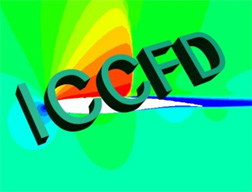
\includegraphics[height=2.0in]{exampleFigure.jpg}
  \caption{This is the logo of ICCFD.}
  \lafi{logo}
\end{figure}


\subsection{Subsection Title Example}

\subsubsection{Sub-subsection Title Example}



%%%% BIBLIOGRAPHY
\bibspacing=\dimen 100
\bibliographystyle{unsrt}
\bibliography{biblio}

\end{document}
